\chapter{Literature Review}
\label{chap:two}

The following chapter
will provide a detailed overview of the existing literature
on cryptocurrencies and machine learning methods.
We also cover the use of \ac{PCA} in time-series data
and the use of web search data in financial applications.
\section{Cryptocurrencies}
\label{sec:crypto}

\subsection{Bitcoin}
In the year 2008, an unknown author with the pseudonym Satoshi Nakamoto introduced the idea of 
a purely peer-to-peer electronic cash system. Interestingly the author mentions 
small casual transactions as something that the current model relying on third-party
financial institutions fails to deliver because of unavoidable transaction costs \cite{Nakamoto2008}. 
In contrast, from today's perspective, Bitcoin is a relatively slow medium for micro-transactions because 
technically the receiver has to always wait for a certain amount of blocks to be mined such that
it becomes statistically unlikely that double-spending has been committed by the payer 
\cite{Conti2018}. This phenomenon
can be demonstrated on the data from \textbf{\href{https://coinmetrics.io/}{coinmetrics.io}} which show
that the mean size of a \ac{BTC} transaction ranges in thousands of USD\$. 
Another important aspect is that 
the miners prioritize transactions with higher fees in the block which introduces considerable costs
to each payment. \cite{Moeser2015} have shown the relationship between the transaction fee 
and the transaction latency meaning the time it takes for the transaction to be almost surely valid.
Even though 
there has been some divergence from the original idea of small transactions all of the security measures
regarding the double spending problem in the original whitepaper have turned out to be relatively 
well-defined in a medium time horizon.


Despite the fact, that Bitcoin is generally regarded as the first cryptocurrency it relies on 
many older ideas and technologies that are mostly referenced in the original whitepaper. First and foremost
stands the conference paper \textit{How to Time-Stamp a Digital Document} \cite{Haber1991} which focuses
on the problem of third parties responsible for verification of digital documents. It makes use of 
an already established family of functions known as hashes that surpass privacy concerns and generally
surpass the need for a third party to be involved in the verification process when combined
with the correct consensus algorithm. They define a hash function as follows:

\begin{defin}[Hash]\label{de:hash}
    This is a family of functions $h: \{0,1\} \rightarrow  {\{0, 1\}}^l $ compressing
bit-strings of arbitrary length to bit-strings of a fixed length l, with the following
properties:
\begin{enumerate}
    \item The functions $h$ are easy to compute, and it is easy to pick a member of the family at random.
    \item It is computationally infeasible, given one of these functions $h$, to find a pair
of distinct strings $x,x'$ satisfying $h(x)=h(x')$. (Such a pair is called a collision for $h$)\cite[see Chapter 4.1]{Haber1991}
\end{enumerate}
\end{defin}

And suggest hashing documents together with the time of their creation.
However, the time-stamping might 
fail if the users can tweak the time of their machines. Interestingly, the authors have already 
mentioned that and introduced the idea of chaining the data together with their metadata sequentially in a long chain 
so that the user can trust that something was not overwritten \cite[see Chapter 5]{Haber1991}. 
This is possible due to the properties of the hash functions.
Meaning that we can concatenate arbitrarily long inputs and always produce a fixed-size output. 
Another significant influence came from b-money which was an idea for an anonymous digital
cash system presented in \cite{Dai1998}. B-money proposed the concept of \ac{PoW}
which is a validation protocol that many cryptocurrencies still use. The idea was to solve
computationally challenging puzzles where it can be determined how much effort was used to do so
\cite[see][pg.~1]{Dai1998}.
However, certain worries were being raised about how to regulate a system if the computational power
of computers is increasing every year \cite[see][pg.~3]{Dai1998}. This has been addressed by Bitcoin
with the regulation of difficulty based on the average time it takes to solve the puzzle 
rather than the difficulty itself \cite[see][pg.~3]{Nakamoto2008}.


Since many characteristics of the network are often being used by researchers such as: 
(\cite{Kukacka2023}, \cite{Kristoufek2023}, \cite{Kubal2022} or \cite{Jay2020}) 
in their research, it is critical to understand the underlying mechanics that form them.
Bitcoin takes a completely adverse approach to the general financial system. Whereas traditionally,
banks and other institutions try to keep every transaction encrypted Bitcoin makes all the 
transactions publicly visible and available but hashing the addresses of the sender and receiver.
The process of sending Bitcoins to someone else essentially means adding a digital signature to the
previous transaction from which you received that money. 
However, as \cite[see Chapter 2][pg.~2]{Nakamoto2008} suggests this only mitigates the privacy concerns
but the double spending risk needs to be dealt with a smarter design.
This is solved by the introduction of the \ac{PoW} algorithm. The idea is that
transactions are collected into blocks by the miners who try to solve a computationally difficult 
task that can only be solved by a brute-force search. It is simply a race to find a hash with a 
certain amount of leading zeros which is adjusted based on the mining power of the network.  
The miners are incentivized by \acs{BTC} price for winning the race and also by the transaction
fees that can be added to each transaction as a reward for being prioritized. 
The leading concept is that the blocks are connected sequentially in a chain through the hash.
If we assume that most of the nodes/miners are honest their profit-maximizing behavior should always be
working on the longest chain and thus transactions that have already been spent do not get included
in the chain. After the puzzle is solved by a node it can be validated by all other nodes
in a linear time and they move on to the next block. Despite that, there remains the risk of 
an attacker forking a malicious block and sending his money back or elsewhere. \cite{Nakamoto2008}
claims that the probability of an attacker catching up (or reaching breakeven from
the memoryless property of Poisson distribution) drops exponentially
with each block if the mining power (probability of solving the puzzle) of the
attacker is lower than the power of honest nodes. This mechanism is the root of the Bitcoin
security. However, it also implies that there is an implicit tradeoff between security and the
desired liquidity of cash. Another important property is that there will ever exist only a limited amount
of 21 million of \ac{BTC}s  which makes it inherently a deflationary currency at least
after all of the \ac{BTC}s are mined. Technically there will be less
as some wallets do get lost together with their contents. Limiting supply 
might be an intentional design choice
to contrast the traditional model where banks issue money and cause inflation.


As cryptocurrencies are a relatively new phenomenon they are currently a frontier topic of academic 
research in many different aspects. They are being studied on multiple levels such as
law, technology, cryptography, security, economics or machine learning. Generally, the area
of economics and machine learning will be of interest as we want to uncover
whether there exist some determinants of the bitcoin price or at least features that can be used 
to estimate the pricing dynamics. We assume that there are theoretically three simplified 
possibilities of the pricing model 
of \ac{BTC} and other cryptocurrencies. Firstly, it might be a purely efficient market 
and the price technically follows a random walk process with a potential drift. 
The second model is that the price is entirely
driven by speculative components and lastly, it might be a combination of speculative and fundamental
components.


\subsection{Ethereum}
At the time of writing according to the data from 
\textbf{\href{https://coinmarketcap.com/}{coinmarketcap.com}}, 
\newline
\ac{ETH} 
is the second cryptocurrency 
based on the market capitalization standing at 318 billion USD. Although, there are a lot of 
similarities with \ac{BTC} the idea behind \ac{ETH} is much more profound and builds an entire
technological infrastructure on top of blockchain which provides easily
scriptable smart contracts. \cite{Tikhomirov2018} defines smart contracts as follows:

\begin{quote}
    \textit{Turing-complete programs that are executed in a 
    decentralized network and usually manipulate digital units of value.}
\end{quote}

We might want to reformulate this definition for the purposes
of this thesis to cover a broader meaning.

\begin{defin}[Smart contract]\label{de:contract}
    A program that is running on the blockchain infrastructure as an endpoint
    with a specific address that other entities on the platform can interact
    with in order to execute a transaction for a cost proportional to the
    number of computational steps. The contract 
    usually has a predefined set of rules which is applied to the input data
    and automatically executes on hold whenever called. This allows developers
    to build applications on top of blockchain infrastructure that is run 
    by the distributed network and grants them the unique benefits
    of the blockchain model.
\end{defin}


According to the original whitepaper, the main purpose of \ac{ETH} was not to
create another cryptocurrency but build a simple-to-use scripting language
that would allow developers to create custom applications running on the blockchain 
that share the benefits of the distributed nature of the system but reduce the 
need for hardware as the transactions are handled by the network and also software
as the transactions can be defined in a few lines of code. Notably it 
describes cryptocurrencies as a state transition system:

\begin{defin}[Digital currency ledger]\label{de:ledger}
    From a technical standpoint, the ledger of a cryptocurrency such as \ac{BTC}
    can be thought of as a state transition system, where there is a 
    \textit{state}
    consisting of the ownership status of all existing coins and a 
    \textit{state transition function} that takes a \textit{state} and a 
    \textit{transaction}
    and outputs a new state \textit{state-new} which is the result.
\end{defin}

In this view, we can understand building smart contracts, see Definition~\ref{de:contract}, 
as creating use case specific \textit{state transition functions} 
(\cite[see Chapter Bitcoin As A State Transition System]{buterin2013ethereum},\cite[see Chapter 2]{Tikhomirov2018}). 

We can observe the fundamental difference in 
philosophy between the \ac{BTC} and \ac{ETH} from their respective 
whitepapers. \ac{ETH} is much 
more focused on its role as an application platform whereas \ac{BTC} was mainly 
intended to work as a currency. The \ac{ETH} whitepaper even
presents many ideas for future applications that might benefit from this framework.
This fact is crucial in understanding the 
underlying price-making mechanics as investments into \ac{ETH} might be 
affected by its perceived potential as a technological product rather than 
a typical currency that might be valued mostly as a medium of exchange. 


Even though there are a lot of similarities in the blockchain architecture, 
there have been many functional and implementation differences. The most notable
is the \ac{ETH} scripting language which is a Turing-complete counterpart
to the \ac{BTC} scripting language that did not support infinite looping 
\cite[see Chapter Scripting]{buterin2013ethereum}. The second fundamental 
implementation variation is that each Ethereum block saves the entire 
\textit{state} of the whole network and thus does not need to store
the whole history of the blockchain. On the contrary, \ac{BTC} 
is doing exactly that, as the blocks are state-unaware and only validate blocks
based on the transactions and the wallet software usually
calculates the balances \cite[see Chapter 2]{Tikhomirov2018}. 
As \cite{buterin2013ethereum} pointed out there
is a workaround that makes this implementation roughly equally efficient 
which utilizes the propagation properties of the Merkle tree with the fact
that only a small part of the state changes with each block allowing for
efficient state change using pointers to the specific branches and leaves of 
this data structure, see Figure~\ref{fig:merkel}. The data are stored
at the bottom of this infrastructure and there is an efficient algorithm
that allows the \ac{ETH} software to reference the affected addresses and paths
leading to them.


\begin{center}
    \begin{figure}[H]
        \centering
            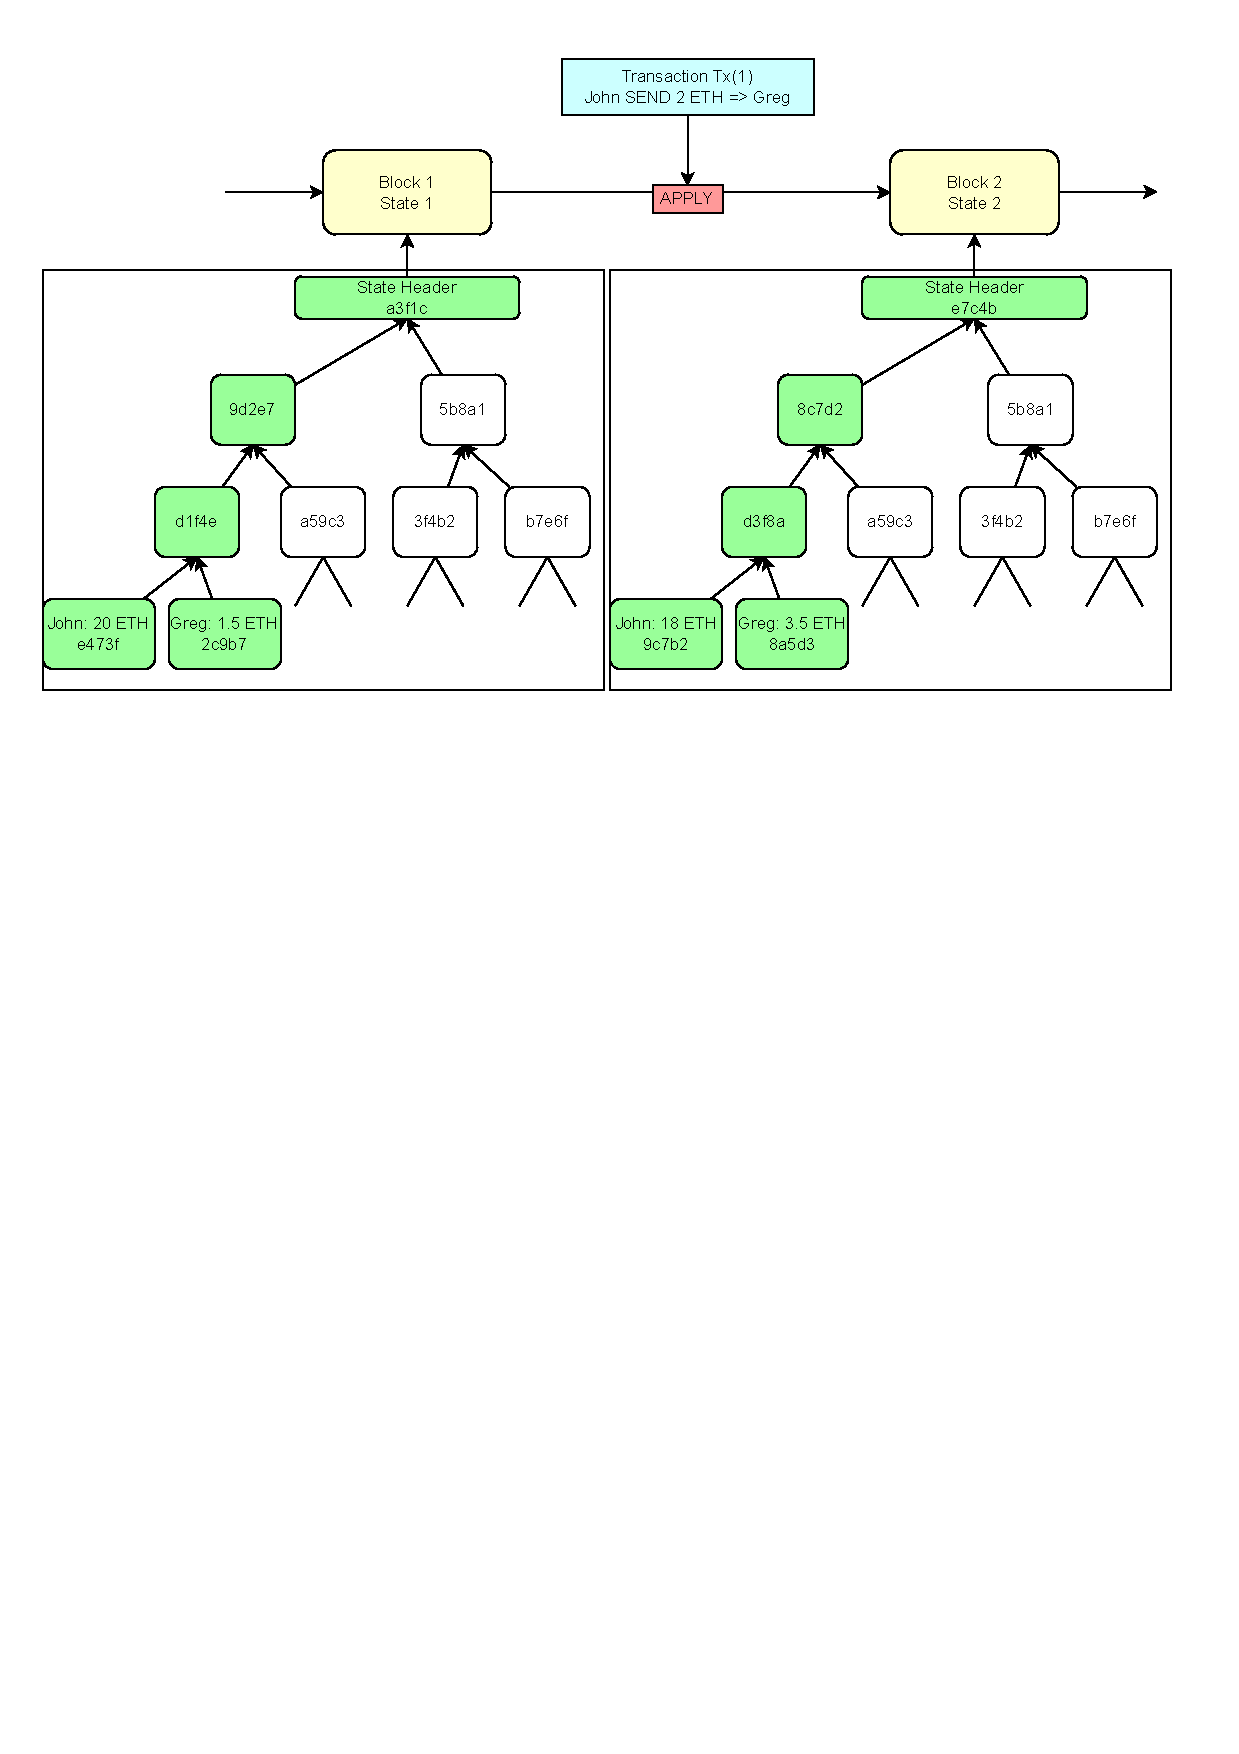
\includegraphics[width=1\textwidth]{Figures/merkle-tree.pdf}
        \caption{Merkel tree with pointers allows efficient state change.}
        \caption*{Source: Author}
        \label{fig:merkel}
    \end{figure}
\end{center}


Lastly, there is a difference in the supply of new coins.
Contrasting the model of \ac{BTC} where the supply is limited \ac{ETH} introduces 
a model of an infinite linear supply of coins to provide incentives 
for future users to join the network as they might still obtain 
new coins and thus limit the wealth concentration common in \ac{BTC} (\cite{buterin2013ethereum}, \cite{Tikhomirov2018}).
Note that \ac{ETH} already switched to the proof-of-stake model in September 2022
but our dataset does not include this period and thus this fact 
is not especially relevant to this thesis.


On the outside \ac{ETH} acts similarly to \ac{BTC}. It is a ledger
that stores the coin balances of accounts where each has a designated unique address.
There are two types of accounts: externally owned accounts which are essentially
the typical users and contract accounts which are the abstraction on top of which
smart contracts can be built with contract code that executes when the account receives
a message from another account (externally owned or a different contract account).
Because of the presence of infinite loops in the scripting language \ac{ETH} employs
a strategy that prevents users from essentially exploiting the Denial-of-service attack.
Nonetheless stands the Halting problem. That can be simplified to the fact
that for a Turing-complete model, there is no way of saying ex-ante whether the program will
halt or run indefinitely. As \cite{Lucas2021} suggests the Halting problem
is usually attributed to Alan Turing's paper 
\cite[On computable numbers, with an application to the Entscheidungsproblem]{turing1936computable},
however, the problem was reformulated in various forms by others. This implies
that this undecidability also holds for any \ac{ETH} contract code.
This is fixed by introducing a gas currency that acts as a cost of computation 
and the maximum has to be predefined in each 
message so that the recipient knows what is at stake \cite{buterin2013ethereum}. 
We can think of this as a type of timeout based on a currency. If gas runs
out all of the state changes are reverted. This also explains the usage 
of the term 
transactions in this setting. 
Transaction typically refers to a set of instructions in SQL or 
other databases that
are bundled together and executed in an all-or-nothing fashion \cite{Kleppmann2017}.
The last important fact, as the whitepaper describes, is that the contract code is run by
all of the miners verifying the block which essentially means applying all of the
transactions and reverting in case of an error.


\subsection{Litecoin}
In comparison to \ac{ETH}, the goal of \ac{LTC} was pronounced from the 
beginning as building a better version of \ac{BTC} that shines where
\ac{BTC} has failed. We might say that \ac{LTC} is a tweaked version of \ac{BTC} with 
different parameters or a hard fork of the \ac{BTC} protocol. 
To our best understanding, the only document that 
is wildly considered the original whitepaper is a transcript of a forum
post by the founder Charlie Lee where he suggests reading 
the \ac{BTC} whitepaper.
Essentially, two main differences address the problems
\ac{BTC} embodies. The first one is faster confirmation time that allows 
\ac{LTC} to be used truly in a fashion that was intended for \ac{BTC} as 
digital cash with high liquidity sacrificing a bit of security. Achieving
that mostly through four times faster block generation. And second one 
is a different proof-of-work algorithm. As \cite{Padmavathi2018} suggests
the intention was most likely since \ac{BTC} mining
was dominated by GPU and ASIC miners which led to a concentration of mining power
in pools and thus more centralized distribution of \ac{BTC}. Despite the initial
promises Litecoin has most likely not fulfilled its envisaged role
and does not currently belong even to the ten most popular cryptocurrencies
by market capitalization.


\section{Machine Learning Methods for Cryptocurrencies}
\label{sec:ml}
Thanks to transformer-based architectures that are the backbone 
of most chatbots. \ac{ML} and artificial intelligence have gotten a lot
of public spotlight during the last two years. However, \ac{ML} methods
have been especially prevalent in research in the last decade.
Particularly in data-driven fields of academia, there have been various
use cases where \ac{ML} shines and outperforms traditional statistical models.
Forecasting has always been an area of interest in many different fields
as the idea of predicting the future based on historical data 
provides intrinsic value in itself.
The field of cryptocurrencies is no exception as the significant volatility
is a thought-provoking problem to tackle and an opportunity to 
win against the rest of the market.


In order to use \ac{ML} or any other data-driven method we implicitly have to 
assume that there are some underlying dynamics of which we can make sense. 
This argument is hard to make without the proper data and might have to be 
studied separately for different time horizons. Thankfully, \cite{Kukacka2023}
argue that some cryptocurrencies especially \ac{BTC} are driven by the interaction of
speculative and fundamental components and thus provide an incentive for us 
to untangle and study these relationships. Disturbingly, even though 
there are many other papers focusing directly on the practical implementation of 
forecasting frameworks for cryptocurrency prices a significant amount of them
do not compare their model to a random walk or other simple statistical model.
We suggest that their approaches should not be condemned but we 
strongly emphasize 
that their results should be interpreted cautiously.

We believe that there is currently an upsetting trend in the studies
focusing on modelling the price or returns of cryptocurrencies using \ac{ML} methods.
There seem to be a lot of inconsistencies in terms of splitting the data
into training and testing sets, making the results robust using some forms 
of cross-validation, comparably presenting the results and 
contrasting the models to a meaningful baseline model. 
This reality arguably contributes to the fact that the results of most of the studies 
are relatively underwhelming and have stagnated in the last few years.
The other side of the coin, arguably worse, are studies that 
present overly optimistic results. A similar critique 
of the generalizability of results was presented by \cite{Akyildirim2020}.
We propose an idea for future research that would imaginably help the field
advance further and stimulate innovation. The suggestion lies in the creation
of a standardized dataset with set splits between train, validation and test data
that would allow for the comparison of different approaches and would
encourage researchers to make their models generalizable. Taking inspiration
from the field of image recognition where the Image-net is a state-of-the-art dataset
to compare models for image recognition. This would allow for a competitive 
environment boosting innovation and development.
We acknowledge that there is a fundamental difference between a dataset
that consists of an unordered series of images and an especially challenging
non-stationary time-series.
Some compromises would undeniably have to be introduced in terms of 
set prediction horizons, different data granularity and artificially set splitting points.
However, there is always a place for variation and this dataset 
could have multiple versions. Even though, this solution is sub-optimal 
we firmly believe the current scattered state of knowledge in this field 
makes it extremely difficult for further development to blossom.


Despite that, we would like to provide a brief overview
of the methods that are often incorporated in price or returns modelling pipelines.
As we already mentioned in order for \ac{ML} to work as a forecasting
algorithm there has to
exist a possibility of drawing information about the future from the past.
That is a non-trivial assumption because it contradicts The Efficient market 
hypothesis
that was formulated for capital markets by \cite{Fama1970}.
It is thus no oddity that \cite{Ren2022} have found out that across 395 scientific
articles about the use of \ac{ML} in cryptocurrencies the most cited 
article was \cite{Urquhart2016} that studied the efficiency of \ac{BTC} and 
concluded that the \ac{BTC} market is inefficient but may become efficient in the future.
And that the keyword
inefficiency was the one with the highest burst of emergence among the articles.


There are generally two types of the problem formulation. Either the price is 
being modelled as a regression problem or the movement of the market is predicted
as a binary classification. Modelling market movement
is easier and it is also much more comparable across studies. If we can assume 
that there are approximately the same amounts of ups and downs we can work
against the 50\% baseline \cite{Akyildirim2020}.
\cite{Khedr2021} pointed out that cryptocurrencies lack seasonal trends
which makes them challenging to predict for traditional statistical models. 
They also distinguish four types of factors influencing cryptocurrency price.
Namely: demand and supply, crypto market, macro-economic and political. 
Our work will cover the first three types of factors as the political factors
are hard to quantify. Later \cite{Ren2022} suggested that future researchers should
study measurement tools for political factors. 
If you want to find out more about research in this
field from 2010-2020 please view \cite{Khedr2021} which provides a comprehensive
review. However, as we suggested 
earlier the aspect of comparison between studies is rather limited.


\cite{Alessandretti2018} compared multiple models from the perspective
of portfolio management comparing them using return on investment and
suggested that all of the \ac{ML} models outperformed the moving average baseline.
They also introduce the idea of predicting cryptocurrencies prices in \ac{BTC} 
rather than USD
to filter out the effect of overall cryptocurrency market growth and ease 
the effects of spurious correlation. In their study \ac{LSTM} outperformed 
the gradient-boosting decision trees with longer time horizons and vice versa.
Lastly, they pinpointed the fact that expressing prices in terms of \ac{BTC}
helped the predictions and concluded that forecasting only the trend of individual 
currencies might be easier than also predicting the overall market trend.
\cite{Chowdhury2020} used ensemble methods to predict the prices of multiple 
cryptocurrencies. Utilizing the fact that combining multiple weaker models
with uncorrelated errors with voting can increase the overall 
performance \cite[see Chapter 14.2]{bishop2006pattern}. 
Unfortunately however impressive their results might seem
they have been evaluated only on a month of predictions which is in our view insufficient.





\section{Principal Component Analysis}
\label{sec:pca}


\subsection{PCA in Time Series}
\ac{PCA} is a widely adopted signal processing technique that is typically
used to lower dimensionality of input features and to mitigate noise in the
signal by transforming the data into a different feature space while ensuring
that the new principal components remain uncorrelated. 
Traditional usecases include dimensionality reduction for visualization purpouses 
(word embedding vectors), noise reduction in ECG, dimensionality reduction for performance reasons
of different \ac{ML} methods and many other signal processing pipelines.


Thanks to its valuable properties it has been recognized also as a tool 
to simplify and bring insights into multivariate time-series data 
concretely in the financial sector. However, using \ac{PCA} in time-series
usually comes with many identified challenges. 
Especially the need for the data to be normalized before being processed by 
the \ac{PCA} layer might turn to be almost impossible to fulfill with
non-stationary time-series. Despite these shortcoming many researchers have 
used \ac{PCA} in their predictive work with a substantial success.


Most notably \cite{Nadkarni2018} designed a technical analysis based trading 
strategy for stocks and indexes that used \ac{PCA} to reduce the dimensionality
of input features from 6 to 31 that enabled the genetic NeuroEvolution algorithm
to design much simpler \ac{ANN}, reduce noise in the data and decrease 
the risk of overfitting the training datasetset. Their approach significantly 
outperformed the Buy and Hold strategy and they conclude that
\ac{PCA} was vital to achieve such results. Their work is especially important 
because of generalizability for future work as their approach used
the broad population of \ac{ANN}s even making each neuron dynamically
choose different activation function and thus introduces no constrains
on the generality of the results. Lastly they concluded that \ac{PCA} 
led to lower
risk, less days spent with capital in the market and higher daily profits.


Similarly, \cite{Chowdhury2018} used \ac{PCA} and Independent Component 
Analysis as a preprocessing layer for stock prediction and 
found out that the proposed framework outperformed the approach 
where only the final \ac{SVR} was used for prediction. Many
other works use \ac{PCA} only as a dimensionality reduction technique
such as \cite{Toledo2022}.


An alternative novel approach used by some researchers  
(\cite{Shah2021}, \cite{mohsin2021}, \cite{Smales2020})
focuses on creating a cryptomarket wide index using \ac{PCA} to 
capture the overall market trends. \cite{Smales2020} found that 
the first principal component explains a large portion of the variation and 
is highly correlated with the \ac{BTC} returns and thus support the notion
of \ac{BTC} returns being an important driver for other cryptocurrencies.
\cite{Shah2021} critique the use of rule based indexes that do not rely
on any fundamental mathematical reasoning and thus create a dynamic index
using \ac{PCA} that captures the overall market trends. However, they 
discourage the use of the index as an ETF highlighting the fact that the 
maximal variance optimization may be associated with higher volatility.


\section{Web Search Data in Financial Applications}


The phenomenon of Google Trends has drawn attention of many researchers.
First and foremost stands the idea of Google Flu Trends. A project
launched by Google which aimed at predicting flu epidemics using the symptom
related searches by the users \cite{Ginsberg2009}. However, as \cite{Lazer2014}
pointed out there have been many underlying issues both in the data construction
and the dynamic nature of the search engine changing with years of development.
We should highligh the importance of the correlation-causation fallacy in
the use of Google Trends or other search based services. It is even worsened
by the Google Trends weekly data granularity which makes it especially challenging 
to assess any kind of causality and its direction. We have to take into
account the possibility that there is a bidirectional influence 
between Google Trends and \ac{BTC} prices. Despite these challenges, research 
suggest that there is an underlying value in using web search data for modelling
financial time series.



\cite{Hu2018} used \ac{ANN} to predict the direction of the stock market
indexes and compare two setups with and without Google Trends and conclude that 
inclusion of Google Trends improves the performance of their models. Similarly,
\cite{Huang2019} studied the effect of investor attention measured by Google Trends
as a potential market signal. Interestingly, they do not find evidence that
market movements cause changes in search volumes. However, they conclude that
search terms are useful in predicting stock market movements
and as a proxy variable for investor attention. Most notably they emphasize 
that the effect is conditional on the sentiment of the search. Suggesting
that we need to distinguish between positive and negative searches. This idea
was adressed before in \cite{Kristoufek2013} that found an asymmetric effect of 
positive and negative searches which were discriminated based on whether 
the price over or underperformed compared to a moving average of 4 days
for Google Trends and 7 days for Wikipedia visits. Furthermore, \cite{Arratia2021}
studied both linear and nonlinear effect between Google Trends and \ac{BTC} returns
and also conclude that Google Trends can be used to improve accuracy when forecasting
\ac{BTC} prices.





